\chapter{シミュレーションにおける実験評価}\label{simulation}

この章では,実験が適切に構築されているか,そしてその際に得られるべき物理量をMonte Carloシミュレーションを用いて評価する.


\section{シミュレーションの意義}

我々の実験では,複雑に物体が組み合わされており,我々が求めるイベントがどれくらいの頻度で発生しうるのかを計算するのは立体角や断面積の計算が入り組みかなり難しい.
そこでMonte Carloシミュレーションを用いて,実験レートを評価する.Geant4を用いてプラスチックシンチレータの中で停止せずに陽電子がターゲットに到達するか,そしてターゲットから発生したガンマ線がNaIシンチレータを光らせるかを確かめることができる.

今回用いた線源は$\ce{^{22}Na}$ の標準線源であり,200 kBqのものである.
この線源強度と我々の実験期間約1週間を考慮して,0.1 Hzの実験レートを目標に実験のデザインが適当か検証した.
本実験でオルソポジトロニウムの寿命を測定する過程の評価を,$\ce{^{22}Na}$ 線源が$\beta$ 崩壊した陽電子がシンチレーターを通過してシリカゲルに到達する過程のレート評価,線源から直接NaIシンチレータに入る$\gamma$ 線の評価,そして形成されたポジトロニウムが崩壊し,放出された$\gamma$ 線がNaIシンチレータで落とすエネルギーの評価の3つに分割してシミュレーションを行った.



\section{プラスチックシンチレーターの通過}

\subsection{概要}
今回の実験で用いられたプラスチックシンチレータは0.15 mmの厚みのものである.線源から放出される陽電子が,シンチレータ内で停止してしまうとシリカゲルに到達せずポジトロニウムを形成することができない.
ポジトロニウムを形成するためには,陽電子がまず標準線源のアルミ窓を通過して,空気中を伝播し,さらにシンチレータをエネルギーを落としきること無く通過する必要がある.
Geant4を用いて実際の線源を含めたジオメトリを作成し,シンチレータと線源の距離を変えながらエネルギーを落としきらず通過してくる粒子の割合を調べた.
このとき,ポジトロニウムのミキシングを起こすために用いる磁場を,陽電子をシリカゲルまで導く用途にも援用する.このときの磁場を,最もターゲットであるシリカゲルまで陽電子を導くのに効率が良い線源窓に垂直な方向に設定し,一様な磁場0.1 Teslaと概算した.この強度については後に考察する.

\subsection{ジオメトリ}

\subsection{陽電子到達数と立体角}

\subsection{結果}

\begin{figure}[htbp]
	\centering
		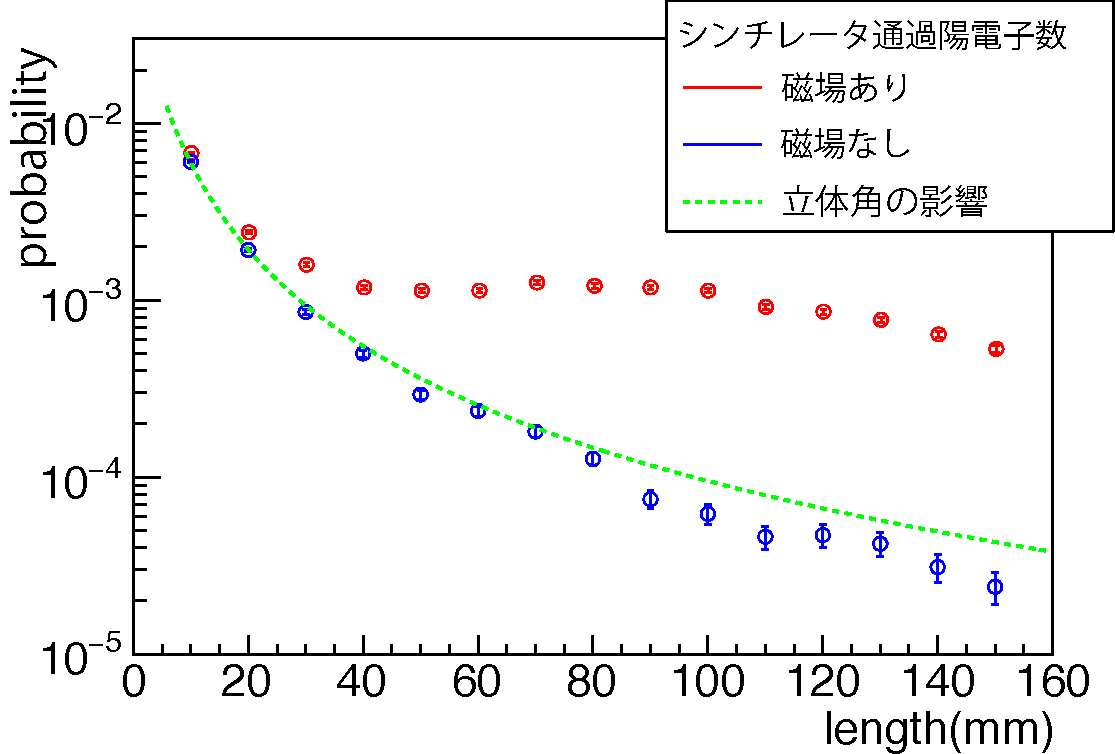
\includegraphics[width=10cm]{fig/scinti_test.pdf}
	\caption{プラスチックシンチレータ通過粒子割合}
	\label{scinti_test}
\end{figure}

\section{崩壊陽電子に対するバックグラウンド評価}

\subsection{ジオメトリ}

\section{予想されるエネルギースペクトル}

